\section{Design interfaces} \label{ch:di}

This chapter discusses the design interfaces. First off, in section \ref{sec:N2} the interfaces between the different subsystems or departments which are considered during the design are given and discussed. This is appended by the design interfaces which needs to be considered during the operation of the mission in the form of a communication flow diagram in section \ref{sec:comflow}.

\subsection{Subsystem design interfaces} \label{sec:N2}
This section defines the interfaces between the different subsystems of the \gls{hiad}. The interfaces are defined in a similar manner as the technical work division of chapter \ref{sec:org}. This subdivision is trajectory \& control, aerodynamics, thermodynamics and structure.  The interfaces are illustrated in the form of a N2 chart as displayed in Fig. \ref{fig:N2} and will subsequently be discussed from the perspective of required inputs per subsystems.

\begin{figure}[H]
\centering
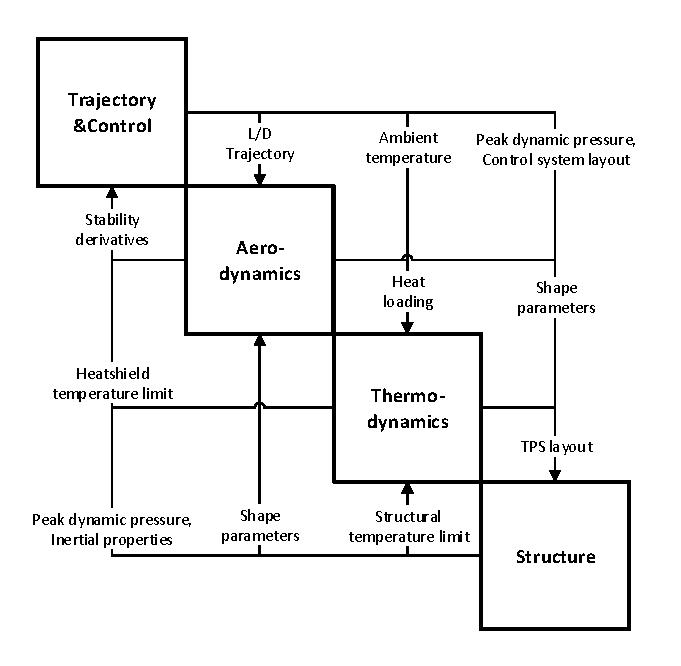
\includegraphics[width = 0.8\textwidth]{Figure/N2.pdf}
\caption{N2 of the interfaces in the \gls{hiad} design}
\label{fig:N2}
\end{figure}

\subsubsection{Trajectory \& Control}

The trajectory and control department or subsystem is one of the main drivers of the requirements. Outputs are mainly derived from the trajectory and control analysis altough the inputs are also of crucial importance. 

The trajectory and control department requires stability derivatives in order to analyse the trajectory possibilities. Stability derivatives are considered in the broadest sense, also including other aerodynamic values such as \gls{sym:CD} \gls{sym:A}, \gls{sym:CL}\gls{sym:A} and \gls{sym:CM}\gls{sym:A} although these values are not actual derivatives. The input from the control department is  best summarized as below.

\begin{itemize}
\item Best if control dep. fills this in.
\item 
\end{itemize}

As the control department and aerodynamic department become integrated the trajectory will be actively controlled in order to stay within the performance limits. For this purpose an additional heat shield temperature limit is required. The temperature limit will function as a constraint on the maximum possible deceleration.

Finally the inertial properties, such as for example the mass moments of inertia, are provided by the structural department which are subsequently combined by the control department for the orbital analysis.

\subsubsection{Aerodynamics}
The aerodynamics department provides two main function. Providing stability derivatives which are required for the orbital calculations, and providing the thermal loads. 
For the former, stability derivatives are again considered in the broadest sense as discussed above. 

The trajectory input is also considered in very broad sense. The full trajectory yields a Machnumber, velocity and atmospheric properties all as a function of time which are required as a input for the Aerodynamic calculations. Note that the atmospheric properties follow from the location in the trajectory via the \gls{nasa} \gls{marsgram} software\cite{Justus2001}.

The actual shape of the system may differ slightly from the specifications as defined by the aerodynamic department itself. As such the aerodynamic department requires additional input from the structural department for the exact shape specification. This can be seen in the N2 chart as rather direct iteration loop between these two subsystems.

\subsubsection{Thermodynamics}
The main inputs for the thermodynamics department is the heat loading as function of time combined with a ambient atmospheric temperature. Moreover a temperature limit is required for the point to which the structure needs to be cooled down. This is value provided by the structure department which joins the \gls{tps} and the payload module.

\subsubsection{Structure}

The structure is sized on the structural loads. These structural loads follow mainly from the peak dynamic pressure and control forces from the trajectory and control department. Moreover from the thermodynamics department a heatshield \gls{tps} layout is defined which need to be fitted onto the structure and needs to be taken into account. 

The control forces are very dependent on the type of control system implemented. As such the type of control system implemented has its inputs on the structural subsystem as well as the applied control forces. 

Finally a shape is defined by the aerodynamics department for which the structure needs to be sized. 

\subsection{System communication flow} \label{sec:comflow}
Communication flow primarily takes place with respect to trajectory sensing and control. In order to adhere to a certain trajectory and to counteract perturbations, alterations in vehicle dynamics are required. These alterations are performed by actuators, as investigated in Chapter \ref{ch:astrocontrol}. The magnitude and direction of the alterations are determined by an on-board computing unit, by a comparison with the actual attitude as provided by attitude sensors mounted on the (re-)entry vehicle. Trajectory and attitude information is communicated to ground control via a Telemetry and Command Unit. A fail-safe system is included to take over computer functions in case of computer failure. This communication flow is depicted in Fig. \ref{fig:comflow}.

\begin{figure}[H]
\centering
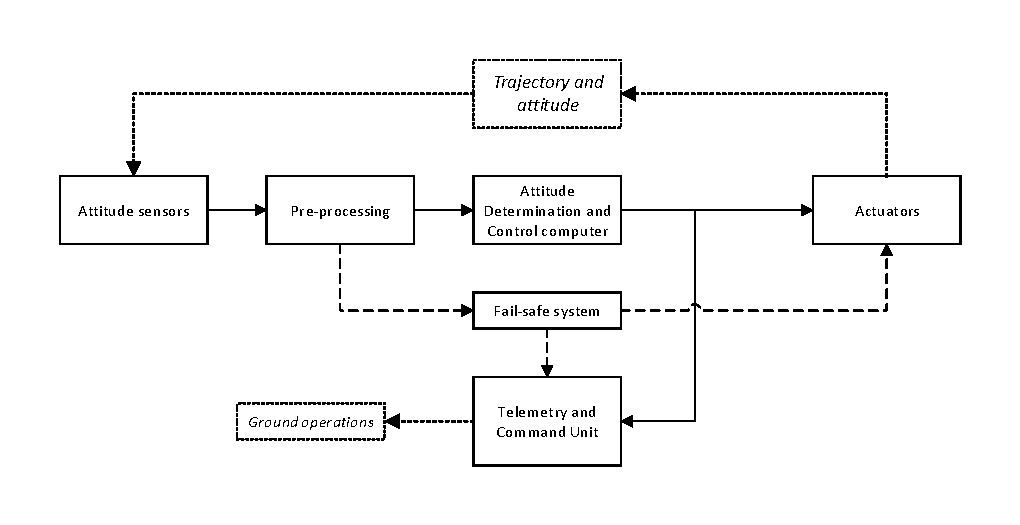
\includegraphics[width = 0.8\textwidth]{Figure/CommunicationChart.pdf}
\caption{Communication flow of control subsystem}
\label{fig:comflow}
\end{figure}

